\section{本章小结}

本章初步定义了一些信号与系统的概念,并举了几个例子。
这些例子涵盖不同的学科,但它们有一个共同的特点,一个输入量通过一个系统的作用产生一个输出量。

\begin{figure}[h]
\centering
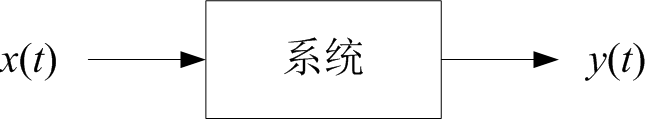
\includegraphics[height=1cm]{1.6-1.png}
\end{figure}

RC电路例子需要特别注意,在今后章节会反复引用。
\begin{figure}[h]
\centering
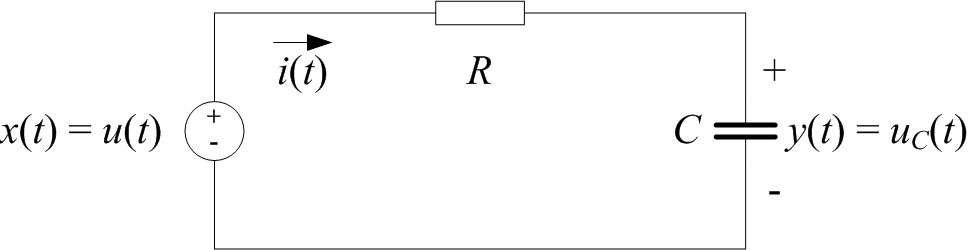
\includegraphics[height=2cm]{1.5.1-1.png}
\end{figure}
\[
\frac{dy}{dt}+\frac{1}{RC}y=\frac{1}{RC}x
\]




